%% Методические указания к выполнению, оформлению и защите выпускной квалификационной работы бакалавра
%% 2.4 Аналитический раздел
%%
%% В данном разделе расчётно-пояснительной записки проводится анализ предметной области и выделяется основной объект исследования.
%% Если формализовать предметную область с помощью математической модели не удается и при этом она сложна для понимания, то для отображения происходящих в ней процессов необходимо использовать методологию IDEF0, а для описания сущностей предметной области и взаимосвязей между ними — ER-модель.
%%
%% Затем выполняется обзор существующих методов и алгоритмов решения идентифицированной проблемы предметной области (опять же с обязательными ссылками на научные источники: монографии, статьи и др.) и их программных реализаций (при наличии), анализируются достоинства и недостатки каждого из них.
%% Выполненный обзор должен позволить объективно оценить актуальное состояние изучаемой проблемы.
%% Результаты проведенного анализа по возможности классифицируются и оформляются в табличной форме.
%%
%% На основе выполненного анализа обосновывается необходимость разработки нового или адаптации существующего метода или алгоритма.
%%
%% Если же целью анализа являлся отбор (на основе четко сформулированных критериев) тех методов и алгоритмов, которые наиболее эффективно решают поставленную задачу, то форма представления результата должна подтвердить обоснованность сделанного выбора, в том числе — полноту и корректность предложенных автором критериев отбора.
%%
%% Одним из основных выводов аналитического раздела должно стать формализованное описание проблемы предметной области, на решение которой будет направлен данный проект, включающее в себя:
%% — описание входных и выходных данных;
%% — указание ограничений, в рамках которых будет разработан новый, адаптирован существующий или просто реализован метод или алгоритм;
%% — описание критериев сравнения нескольких реализаций метода или алгоритма;
%% — описание способов тестирования разработанного, адаптированного или реализованного метода или алгоритма;
%% — описание функциональных требований к разрабатываемому программному обеспечению,
%% при этом в зависимости от направления работы отдельные пункты могут отсутствовать.
%%
%% Если в результате работы будет создано программное обеспечение, реализующее большое количество типичных способов взаимодействия с пользователем, необходимо каждый из этих способов описать с помощью диаграммы прецедентов [4, 5].
%%
%% Рекомендуемый объём аналитического раздела 25—30 страниц.

\chapter{Аналитический раздел}

\section{Предметная область}

В работе рассматриваются технические устройства, состоящие из некоторого количества источников и приёмников излучения.
Примерами таких устройств (рис. \ref{img:lamp-1}—\ref{img:lamp-2-3}) служит \cite{lighting-engineering, lasers, neodymium-glass-lasers, sarychev}:
\begin{itemize}
	\item различная осветительная, сигнальная техника,
	\item системы некогерентной оптической накачки,
	\item разнообразные излучательные имитаторы,
	\item волоконно-оптические нагревательные печи,
	\item фотонные импульсные генераторы,
	\item облучательные установки, МГД-генераторы и ДДП.
\end{itemize}

\imgp{width=0.85\linewidth}{lamp-1}{Система накачки с дисковыми активными элементами}
\imgp{width=0.9\linewidth}{lamp-2-3}{Объёмная фотохимическая установка и лампа с системой излучающих оболочек}

\imgp{width=0.85\linewidth}{krypton-efficiency}{Спектральное распределение КПД излучения разряда в криптоне. Внутренний радиус разрядной трубки $R=0,3$ см, рабочее давление в разряде $p=2,5$ МПа. \\
	а — ток $I=100$ А, средняя удельная электрическая мощность $\langle w \rangle = 8,5$ кВт/см$^3$, осевая температура плазмы $T_0=9980$ К; \\
	б — ток $I=400$ А, $\langle w \rangle = 62$ кВт/см$^3$ $T_0=11640$ К; \\
	в — ток $I=800$ А, $\langle w \rangle = 170$ кВт/см$^3$ $T_0=12870$ К}

% NOEDITEDNEXTLINE
Последние предназначены для технологического использования фотобиологического, фотохимического, фотолюминесцентного, фотоэлектрического действий оптического излучения ультрафиолетового, видимого и инфракрасного спектральных диапазонов и отличаются особенным многообразием как по конструкции, так и по функциональному назначению.

В общем случае такие системы имеют довольно сложную конфигурацию, состоящую из:
отражателей самой разнообразной формы, различных сред, приёмников и источников излучения, а также полупроводниковых пластин, лакокрасочных покрытий, активной лазерной среды и~др.
В зависимости от длины волны излучения материалы перечисленных элементов по-разному проявляют свои физико-оптические свойства.
На границах разделов сред могут происходить рассеивающее, зеркальное или смешанное отражение, преломление и поглощение.
К тому же вся система находится в едином электромагнитном поле, а источниками излучения могут выступать несколько активных элементов.

Активные излучающие источники состоят из плазменной разрядной трубки и могут быть окружены газово-жидкостным охлаждающим слоем.
В то же время оболочки трубок сами могут быть источниками электромагнитного излучения (рисунок \ref{img:lamp-2-3}).
Поглощение оптического излучения происходит селективно и зависит от материала оболочки (поликор, лейкосапфир, кварц).
В дополнении к этому само покрытие трубок может быть поглощающим или отражающим с задачей разного рода фильтрации спектральных компонент.

Режим работы излучателя определяется огромным количеством элементарных электромагнитных процессов, помимо этого зависит от конфигурации всей системы: геометрии, состава, давления и~т.~д.
Результирующие световое излучение меняется не только в зависимости от спектрального диапазона, но даже в пределах единичного импульса электрического разряда.
В качестве примера на рисунке \ref{img:krypton-efficiency} изображена зависимость кривых спектральных излучений разряда криптона от температуры в плазме, силы и мощности электрического тока.

Таким образом, объектом исследования являются математические модели систем с разрядными источниками мощного селективного излучения и реализующие эти модели программно-алгоритмические средства.
Указанные системы могут быть идентифицированы как системы, назначением и основой функционирования которых является интенсивное электромагнитное воздействие на материалы, среды и процессы.
Речь идёт о системах накачки лазеров, различного типа облучательных установках, технологических процессах, базирующихся на фотохимическом и фотобиологическом действиях света, светотехнических устройствах самого широкого назначения и~т.~д.

\section{Существующие методы моделирования световых систем}

\subsection{Зональный метод}

В основе зонального метода лежит разбиение неизотермического газа и обрамляющего его оболочку на некоторое ограниченное количество малых объёмов и площадей, которые в свою очередь могут считаться практически изотермическими.
Далее для каждого малого геометрического участка моделируемой среды прописывается уравнение энергитического баланса.
Полученная система нелинейных уравнений решается относительно тепловых потоков и температур различными численными методами.

Чисто математически метод не является элегантным, однако прикладное приложение оказывается довольно полезным.

Вполне детализированное изложение метода присутсвует в работе Хоттеля \cite{hottel-1}.
Он же \cite{hottel-2} и независимо от него Эйнштейн \cite{einstein-1, einstein-2} воспользовались методом для моделирования трёхмерных световых термодинамических систем.

Преимущество зонального метода по сравнению, например, с методом Кертиса~— Годсона, состоит в том, что рассматриваемый метод позволяет моделировать системы с неорпеделённым распределением температур в газообразной среде.

\imgh{width=0.65\linewidth}{ziegel-17-18}{Излучение от объёма газа $V_\gamma$ к поверхности $A_k$}

Зональный метод заключается в решении систем уравнений теплового баланса, для условно изотермического объёма $V_\gamma$ (рисунок \ref{img:ziegel-17-18}) с постоянными свойствами, ограниченной поверхностью $A_k$, уравнение записывается в виде:

\begin{equation}
	4a\sigma T^4_\gamma V_\gamma = \sum_{\gamma^* = 1}^{\Gamma} \sigma T^4_{\gamma^*} \overline{g_{\gamma^*} g_\gamma} + \sum_{k=1}^{N} q_{0, k} \overline{g_\gamma s_k},
\end{equation}

\noindent где
\begin{itemize}
	\item $a$ — постоянный коэффициент поглощения газа;
	\item $\Gamma$ — количество конечных объёмов, на которые разделён газ;
	\item $N$ — количество конечных площадей, на которые разделена поверхность;
	\item $\sigma$ — постоянная Стефана — Больцмана;
	\item $T_\gamma$ — абсолютная температура газа $\gamma$;
	\item $q_{0, k}$ — плотность потока излучения, падающего на поверхность $k$;
	\item $\displaystyle \overline{g_{\gamma^*} g_\gamma} \equiv \frac{a^2}{\pi} \int\displaylimits_{V_\gamma} \int\displaylimits_{V_{\gamma^*}} \frac{\tau(S_{\gamma^*-\gamma}) \,\mathrm dV_{\gamma^*} \,\mathrm dV_\gamma}{S^2_{\gamma^*-\gamma}}$ — взаимная поверхность обмена излучения между двумя газами $\gamma^*$ и $\gamma$;
	\item $\displaystyle \overline{g_\gamma s_k} \equiv \frac a\pi  \int\displaylimits_{V_\gamma} \int\displaylimits_{A_k} \frac{\cos{\beta_k}}{S^2_{\gamma-k}} \tau (S_{\gamma - k}) \,\mathrm dA_k \, \mathrm dV_\gamma$ — взаимная поверхность обмена излучения между газом $\gamma$ и поверхностью $k$;
	\item $\tau(S)$ — пропускательная способность площадки $S$.
\end{itemize}

Рассмотренный метод моделирования продолжил своё развитие в дальнейших работах Хоттеля \cite{hottel-1, hottel-2}.
Спектральная зависимость свойств газообразной среды, к сожалению, не учитывается в оригинальном изложении метода, однако существует способ её предусмотрения приближённым способом за счёт введения так называемого среднего коэффициента поглощения между каждой зоной.

Для достижения лучшей точности моделирования при наличии внушительных термальных градиентов Эйнштейн уточнил коэффициенты $\overline{gs}$ и $\overline{gg}$ в работах \cite{einstein-1, einstein-2}.

Приближённый зональный метод, в том числе и его модификации, не подходит для моделирования систем, в которых коэффициент оптического поглощения среды варьируется исходя из температуры.

\subsection{Метод обобщённых угловых коэффициентов}
% https://www.mathnet.ru/links/a952b34718d7ca99449ea74fd103b2bd/tvt43.pdf

В методе обобщённых угловых коэффициентов так же, как и в зональном методе, моделируются системы, состоящие из серого газа и абсолютно чёрной оболочки.

В основе моделирования — уравнение количества тепла, передаваемое от площадки $F_i$ на площадку $F_k$ в единицу времени:

\begin{equation}
	Q_{ik} = (E_i - E_k) F_i \psi_{ik} \; [\text{Вт}],
\end{equation}

\noindent где
\begin{itemize}
	\item $E = 5,77 \cdot 10^{-8} T^4 \; [\text{Вт}/\text{м}^2]$ — плотность полусферического чёрного излучения;
	\item $T$ — абсолютная температура;
	\item $\psi_{ik}$ — отношение количества тепла, достигающего площадки $F_k$, к общему количества тепла, излучаемому площадкой $F_i$.
\end{itemize}

Название «обобщённый угловой коэффициент» для $\psi_{ik}$ впервые введено в работе Невского \cite{nevskiy} благодаря тому, что коэффициент $\psi_{ik}$ учитывает не только сугубо геометрические свойства моделируемой системы, но и поглощение излучения в среде.

В средах, прозрачных для лучистой энергии (так называемых диаметрических средах), выполняется тождественное равенство «обобщённого» и «обыкновенного» угловых коэффициентов:

\begin{equation}
	\psi_{ik} = \varphi_{ik}.
\end{equation}

При осуществлении обмена теплом между площадкой $F_k$ и элементарной площадкой $\mathrm dF_i$, локальное количество тепла определяется соотношением:

\begin{equation}
	\mathrm dQ_{dik} = (E_i - E_k) \psi_{dik} \,\mathrm dF_i,
\end{equation}

\noindent где $\psi_{dik}$ — локальный обобщённый угловой коэффициент, который связан со средним обобщенным угловым коэффициентом $\psi_{ik}$ уравнением:

\begin{equation}
	\psi_{ik} = \frac{1}{F_i} \int\displaylimits_{F_i} \psi_{dik} \,\mathrm dF_i.
\end{equation}

Для световых систем, состоящих их неограниченно протяжённых цилиндрических излучателей, в работе \cite{mikk} с приемлемой точностью были вычислены обобщённые угловые коэффициенты.

В качестве примера некоторые из результатов этой работы представленны в таблице \ref{tbl:mikk}.
Входящие в формулы обобщённых угловых коэффициентов вспомогательные функции оптической плотности среды $N_1$, $N_2$ и $S_1$ так же взяты из \cite{mikk}.

\def\wA{50mm}
\def\wB{55mm}
\def\wC{52mm}
\begin{FixLineStretch}
	\begin{table}[h]
		\small
		\caption{Формулы обобщенных угловых коэффициентов}
		\label{tbl:mikk}
		\begin{tabular}{|p{\wA}|p{\wB}|p{\wC}|}
			\hline
			\TableHeader{\wA}{Расчётная схема попер. сечения системы} & \TableHeader{\wB}{Формула обобщенного углового коэффициента}                                                                                                                    & \TableHeader{\wC}{Формула обыкновенного углового коэффициента}                              \\ \hline
			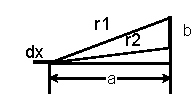
\includegraphics[width=50mm]{inc/img/mikk-1}              & \vspace{-20mm} \[ \psi_{dx, b} = \frac a2 \left[\frac{N_1(kr_2)}{r_2} - \frac{N_1(kr_1)}{r_1}\right] \]                                                                          & \vspace{-20mm} \[ \varphi_{dx, b} = \frac a2 \left(\frac{1}{r_2} - \frac{1}{r_1}\right)\] \\ \hline
			\vspace{1mm}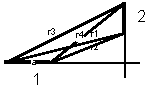
\includegraphics[width=50mm]{inc/img/mikk-2}  & \vspace{2mm} \begin{gather*} \psi_{1,2} = \frac{1}{2ka} [N_2(kr_2) + N_2(kr_3) - \\ - N_2(kr_1) - N_2(kr_4)] \end{gather*}                                                       & \vspace{5mm} \[ \varphi_{1,2} = \frac{1}{2a} (r_1 + r_4 - r_2 - r_3) \]                   \\ \hline
			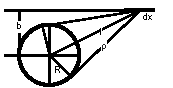
\includegraphics[width=50mm]{inc/img/mikk-3}              & \vspace{-25mm} \begin{gather*} \psi_{dx, l} = \frac{Rh}{\rho^2} \left[ \frac{\rho - R}{\rho} M(k\rho - kR) \right. \\ \left. + \frac R\rho S_1(k\rho - kR) \right] \end{gather*} & \vspace{-13.5mm} \[ \varphi_{dx, l} = \frac{Rh}{\rho^2} \]                                \\ \hline
		\end{tabular}
	\end{table}
\end{FixLineStretch}
\let\wC\relax
\let\wB\relax
\let\wA\relax

Моделирование световых полей методом обобщённых угловых коэффициентов генерирует результаты приемлемой точности в том случае, если излучатель рассматривается как бесконечного протяжённый по какому-то определённому направлению.

Такому случаю на практике соответствуют лучистые системы с пренебрежительно малыми фото-тепловыми эффектами на границах излучающего объёма цилиндра.

По своему принципу метод схож с зональным, поэтому обладает всё теми же недостатками.

\subsection{Метод дискретных ординат}

Моделирование световых полей методом дисретных ординат и соответствующие ему приближённые численные методы решения уравнения теплового переноса широко используются в теплогидравлических и гидродинамических расчётах.

В основе метода дискретных ординат, в отличие от метода обобщённых угловых коэффициентов, лежит то, что угловое лучистое распределение фотонов оценивается в различных дискретных направлениях.

При рассмотрении исчерпывающего числа направлений метод дискретных ординат позволяет получить решение уравнение лучистого переноса энергии с любой желаемой точностью.
Ограничениями в этом случае выступают лишь возможности электронно-вычислительных машин.

Моделирование реальных свето-излучающих систем методом дискретных ординат осуществляется за счёт многократного группового приближения дискретных переменных переноса энергии на соответствующей дискретной трёхмерной сетке.
Следовательно, и пространнственная переменная $r$, и направление $\Omega$, и энергия $E$, и угловые коэффициенты считаются дискретными.

Использование метода дискретных ординат сопряжено с рядом трудностей, которые, ожидаемо, не имеют единственного верного решения. К таким проблемам можно отнести,
\begin{enumerate}
	\item непосредственный выбор дискретных направлений;
	\item приближение интегральных членов по угловой переменной, представленных в уравнения теплового переноса;
	\item приближение производных по компонентам угла $\Omega$ от пучка фотонов, представленных в уравнении теплового переноса в криволинейных системах координат.
\end{enumerate}

\subsection{Диффузно-лучевой метод}

Диффузно-лучевой метод, описанный в работе \cite{gradov-dissertation}, широко использовался для моделирования процессов в значительном количестве тепло-световых систем различной конфигурации \cite{gradov-machine-modeling}.
По целому ряду параметров было проведено сравнение соответствия экспериментальных данных.
Например, для мультиламповой световой разрядной системы с плоскими действующими компонентами результаты моделирования диффузно-лучевым методом должным образом соответствуются с результатами экспериментов по люминесцентным параметрам, что отражено в работах \cite{gradov-calculation-methods, gradov-machine-modeling}.

Суть метода, изложенного в \cite{gradov-dissertation}, заключается в моделировании трехмерного геометрического предстваления системы и использовании видоизменненного алгоритма трассировки лучей, где по всей траектории следования фотонов выполняются различные физико-оптические расчёты.

Наряду с объективными преимуществами метода по сравнению с предшествующими, достигнутыми за счёт принципиально нового способа моделирования световых систем сложной конфигурации, есть ряд недостатков, которые освещены в следующем пункте работы.

\subsection{Сравнительный анализ существующих методов моделирования световых систем}

\def\wA{5mm}
\def\wB{28mm}
\def\wC{23mm}
\def\wD{23mm}
\def\wE{23mm}
\def\wF{23mm}
\def\wG{23mm}
\def\wH{22mm}
\def\wI{22mm}
\def\wJ{22mm}
\begin{FixLineStretch}
\begin{sidewaystable}[p]
	\small
	\caption{Сравнительный анализ существующих методов моделирования световых полей}
	\label{tbl:existing-modeling-methods}
	\begin{tabular}{|p{\wA}|p{\wB}|p{\wC}|p{\wD}|p{\wE}|p{\wF}|p{\wG}|p{\wH}|p{\wI}|p{\wJ}|}
		\hline
		\TableHeader{\wA}{№} & \TableHeader{\wB}{Метод}                                                                                & \TableHeader{\wC}{Учёт излучения плазмы источника из объёма} & \TableHeader{\wD}{Учёт неоднородного распределения параметров плазмы по объёму} & \TableHeader{\wE}{Нахождение распределения поглощённой мощности по объёму плазмы} & \TableHeader{\wF}{Использование параллельных алгоритмов} & \TableHeader{\wG}{Возможность применения метода для построения замкнутых систем моделирования} & \TableHeader{\wH}{Универсальность подходов для расчёта систем с плазмой произвольной оптической плотности} & \TableHeader{\wI}{Отсутствие вероятностного розыгрыша лучей} & \TableHeader{\wJ}{Доступность ПМО и ЭВМ} \\ \hline
		1                    & \everypar{\hspace*{0pt}} Зональный \cite{radiation-heat-transfer}                                       & Нет                                                          & Нет                                                                             & Нет                                                                               & Да                                                       & Нет                                                                                            & Нет                                                                                                        & Да                                                           & Нет                                      \\ \hline
		2                    & \everypar{\hspace*{0pt}} Обобщённых угловых коэффициентов \cite{encyclopedia-of-low-temperature-plasma} & Нет                                                          & Нет                                                                             & Нет                                                                               & Да                                                       & Нет                                                                                            & Нет                                                                                                        & Да                                                           & Нет                                      \\ \hline
		3                    & \everypar{\hspace*{0pt}} Дискретных ординат \cite{surzhikov}                                            & Да                                                           & Нет                                                                             & Нет                                                                               & Да                                                       & Да                                                                                             & Нет                                                                                                        & Да                                                           & Нет                                      \\ \hline
		4                    & \everypar{\hspace*{0pt}} Диффузно-лучевой \cite{gradov-dissertation}                                   & Да                                                           & Да                                                                              & Нет                                                                               & Нет                                                      & Да                                                                                             & Да                                                                                                         & Нет                                                          & Да                                       \\ \hline
	\end{tabular}
\end{sidewaystable}
\end{FixLineStretch}
\let\wJ\relax
\let\wI\relax
\let\wH\relax
\let\wG\relax
\let\wF\relax
\let\wE\relax
\let\wD\relax
\let\wC\relax
\let\wB\relax
\let\wA\relax

В таблице \ref{tbl:existing-modeling-methods} представлены результаты сравнения существующих методов по некоторым важным критериям для современного физико-математического моделирования световых полей сложной конфигурации.

Видно, что по предложенным критериям диффузно-лучевой метод из работы \cite{gradov-dissertation} смотрится наиболее выигрышно относительно остальных, однако, несмотря на это, всё ещё обладает рядом мест, в которых имеется возможность произвести улучшение.

Исходя из анализа, актуальным и перспективным направлением термодинамического моделирования световых полей является разработка метода, лишённого пробелов по перечисленным в таблице \ref{tbl:existing-modeling-methods} критериям.

\section{Формализация задачи}

На рисунке \ref{img:01_A0} представлена диаграмма IDEF0 дискретно-лучевого метода моделирования световых полей в системах с неоднородными поглощающими и излучающими средами на основе параллельных вычислений.

\img{width=\linewidth}{01_A0}{Диаграмма IDEF0 дискретно-лучевого метода моделирования световых полей сложной конфигурации}

Входными данными метода являются физико-оптические свойства системы, а именно:
\begin{itemize}
	\item геометрия системы — список поверхностей сред системы;
	\item распределение температур в средах — список функций распределений;
	\item распределение коэффициента оптического поглощения в средах~— список функций распределений;
	\item коэффициенты отражения поверхностей моделируемых сред~— список коэффициентов;
	\item коэффициенты преломления — список коэффициентов;
	\item моделируемые частоты разрядного светового излучения~— список частот.
\end{itemize}

Выходными данными является распределение удельной и объёмной поглощённых мощностей светового излучения в средах неоднородной системы.

% TODO(a.kerimov)
Ограничения:
\begin{itemize}
	\item формы поверхностей сред~— бесконечно протяжённые цилиндрические симметрии;
	\item выбор частот светового излучения из заданного дискретного списка частот;
	\item ограниченный набор материалов.
\end{itemize}

\section*{Выводы}

В аналитическом разделе выпускной квалификационной работы был проведён анализ предметной области и выделен объект исследования.

Затем был проведён обзор существующих методов моделирования световых полей в системах сложной конфигурации, проанализированы их достоинства и недостатки, а результаты были классифицированы и оформлены в табличном виде.

В заключении раздела задача была формализована, определены входные и выходные данные метода и его ограничения.
